\makeheading{Week 7}{\daterange{2021-10-27}{2021-11-03}}%chktex 8
\section{Two Interesting Applications}
\subsection{Interesting Application \#1: The Galton-Watson Branching Process}
\begin{itemize}
      \item The famous \emph{Galton-Watson Branching Process} was first introduced by Francis Galton in 1889
            as a simple mathematical model for the propagation of family names.
      \item They were reinvented by Leo Szilard in the late 1930s as models for the proliferation of free
            neutrons in a nuclear fission reaction.
      \item Such mathematical models (and their generalizations) continue to play an important role in
            both the theory and applications of stochastic processes.
\end{itemize}
\subsubsection{The Galton-Watson Branching Process}
\begin{itemize}
      \item In what follows, we assume that a population of individuals (which may represent people,
            organisms, free neutrons, etc.) evolves in discrete time. Specifically, we define:
            \begin{align*}
                  X_0 & \equiv \text{population of the $0\textsuperscript{th}$ (original) generation}, \\
                  X_1 & \equiv \text{population of the $1\textsuperscript{st}$ generation},            \\
                      & \vdotswithin{\equiv}                                                           \\
                  X_n & \equiv \text{population of the $n\textsuperscript{th}$ generation},            \\
                      & \vdotswithin{\equiv}
            \end{align*}
      \item We assume that each individual in a generation produces a random number (possibly $0$) of
            individuals, called offspring, which go on and become part of the very next generation.
      \item In other words, it is always the offspring of a current generation which go on to form the next
            generation.
      \item We further assume that individuals produce offspring independently of all others according to
            the same probability distribution, namely
            \[ \alpha_m=\Prob{\text{an individual produces $ m $ offspring}},\; m=0,1,2,\ldots. \]
      \item In addition, for purposes we will see later, we assume that $ \alpha_0\in(0,1) $ and $ \alpha_0+\alpha_1<1 $.
      \item For $ j\in\mathbb{N} $, let $ Z_i^{(j)} $ be the number of offspring produced from individual $ i $ in the
            $ j\textsuperscript{th} $ generation.
      \item Due to the earlier independence assumptions, $ \Set{Z_i^{(j)}}_{i=1}^\infty $ is an iid sequence of rvs with
            $ \alpha_m=\Prob{Z_i^{(j)}=m} $ for any $ j\in\mathbb{N} $. Moreover, let $ \mu=\E{Z_i^{(j)}} $ and
            $ \sigma^2=\Var{Z_i^{(j)}} $ represent the (common) mean and variance, respectively, of the number of offspring produced by a single
            individual.
      \item Based on the above assumptions, the Galton-Watson process $ \Set{X_n,n\in\mathbb{N}} $ is actually a DTMC
            taking values in the state space $ \mathcal{S}=\mathbb{N} $, since it follows that
            \[ X_n=\sum_{i=1}^{X_{n-1}} Z_i^{(n-1)},\label{eq3.9}\tag*{(3.9)} \]
            implying that the Markov property and stationarity assumption are both satisfied.
      \item In this DTMC, we remark that $ P_{0,0}=1 $, since state $0$ is obviously an absorbing state.
      \item If we now consider state $ i $, $ i\in\mathbb{Z}^+ $, then we can easily show that state $ i $ is transient as follows:
            \begin{itemize}
                  \item Clearly, states $ 0 $ and $ i $ do not communicate.
                  \item Note that $ P_{i,0}=\alpha_0^i>0 $ (since $ \alpha_0>0 $).
                  \item By the contrapositive of Theorem 3.5, state $i$ must therefore be transient.
            \end{itemize}
      \item Thus, since state $0$ is recurrent and states $ 1,2,3,\ldots $ are transient, the following conclusion can
            be drawn: \emph{The population will either die out completely or its size will grow indefinitely (to $ \infty $)}.
      \item \textbf{We have}: $ X_n=\sum_{i=1}^{X_{n-1}} Z_i^{(n-1)} \leftarrow $~\ref{eq3.9}.
      \item Since~\ref{eq3.9} infers that $X_n$ is expressible as a \emph{random sum}, we can apply the results of Example
            2.9 to obtain
            \[ \E{X_n}=\mu\E{X_{n-1}} \]
            and
            \[ \Var{X_n}=\sigma^2\E{X_{n-1}}+\mu^2\Var{X_{n-1}}. \]
      \item For convenience, let us henceforth assume that $X_0 = 1$ (with probability $1$). As it is
            understood that $X_0 = 1$, for ease of notation, we will suppress writing the condition ``$X_0 = 1$''
            in all expectations and probabilities which follow.
\end{itemize}
\subsubsection{The Galton-Watson Branching Process: Mean}
\begin{itemize}
      \item \textbf{We have}: $ \E{X_{n}}=\mu \E{X_{n-1}} $, $ X_0=1 $ with probability $1$.
      \item Now, let us consider $ \E{X_n} $ for several values of $ n $:
            \begin{align*}
                   & \text{Take }n=1\implies \E{X_1}=\mu\E{X_0}=\mu,   \\
                   & \text{Take }n=2\implies \E{X_2}=\mu\E{X_1}=\mu^2, \\
                   & \text{Take }n=3\implies \E{X_3}=\mu\E{X_2}=\mu^3.
            \end{align*}
            Based on the above findings, it is straightforward to deduce that $ \E{X_n}=\mu^n $, $ n\in\mathbb{N} $.
\end{itemize}
\subsubsection{The Galton-Watson Branching Process: Variance}
\begin{itemize}
      \item \textbf{We have}: $ \Var{X_n}=\sigma^2\E{X_{n-1}}+\mu^2\Var{X_{n-1}} $, $ X_0=1 $ with probability $ 1 $.
            Similarly, we have
            \begin{align*}
                   & \text{Take }n=1\implies \Var{X_1}=\sigma^2\E{X_0}+\underbrace{\mu^2\Var{X_0}}_{0}=\sigma^2,                 \\
                   & \text{Take }n=2\implies \Var{X_2}=\sigma^2\E{X_1}+\mu^2\Var{X_1}=\sigma^2\mu+\sigma^2\mu^2,                 \\
                   & \text{Take }n=3\implies \Var{X_3}=\sigma^2\E{X_2}+\mu^2\Var{X_3}=\sigma^2\mu^2+\sigma^2\mu^3+\sigma^2\mu^4.
            \end{align*}
            Continuing inductively, we find that
            \[ \Var{X_n}=\sigma^2\mu^{n-1}\sum_{i=0}^{n-1} \mu^i,\; n\in\mathbb{N}, \]
            which simplifies to give
            \[ \Var{X_n}=\begin{cases*}
                        n\sigma^2,                                           & \text{if $ \mu=1 $},  \\
                        \sigma^2\mu^{n-1}\bigl(\frac{1-\mu^n}{1-\mu} \bigr), & \text{if $\mu\ne 1$}.
                  \end{cases*} \]
\end{itemize}
\subsubsection{The Galton-Watson Branching Process: Extinction Probability}
\begin{itemize}
      \item Under the assumption that $ X_0=1 $, let $ \pi_0 $ denote the limiting probability that the population dies out.
            In other words,
            \[ \pi_0=\lim\limits_{{n} \to {\infty}} \Prob{X_n=0}. \]
      \item Let us first consider the situation when $ \mu<1 $, which is referred to as the \emph{subcritical} case.
            Clearly, as $ n\to\infty $, $ \E{X_n}=\mu^n $ and $ \Var{X_n}=\sigma^2\mu^{n-1}\bigl(\frac{1-\mu^n}{1-\mu}\bigr) $ both converge to $ 0 $.
            Therefore, we would expect that if $ \mu<1 $, then $ \pi_0=1 $. To prove this formally, note that
            \[ \mu^n=\E{X_n}=\sum_{j=1}^{\infty} j\Prob{X_n=j}\ge \sum_{j=1}^{\infty} 1\cdot \Prob{X_n=j}=\Prob{X_n\ge 1}=1-\Prob{X_n=0}. \]
            This implies that $ 1-\mu^n\le \Prob{X_n=0}\le 1 $. Taking the limit as $ n\to\infty $ leads to:
            \[ \lim\limits_{{n} \to {\infty}} (1-\mu^n)\le \lim\limits_{{n} \to {\infty}} \Prob{X_n=0}\le \lim\limits_{{n} \to {\infty}} 1\implies 1\le \pi_0\le 1, \]
            or simply, $ \pi_0=1 $.
      \item On the other hand, suppose that $ \mu\ge 1 $. By conditioning on the number of offspring produced
            by the single individual present in the population at time $0$, we obtain
            \[ \pi_0=\Prob{\text{population dies out}}=\sum_{j=0}^{\infty} \Prob{\text{population dies out}\given X_1=j}\alpha_j. \]
            However, with $ X_1=j $, the population will eventually die out iff each of the $j$ families started
            by the members of the first generation eventually dies out.

            As each family is assumed to act independently, and since the probability that any particular
            family dies out is simply $ \pi_0 $, it follows that $ \Prob{\text{population dies out}\given X_1=j}=\pi_0^j $ and our above
            equation becomes
            \[ \pi_0=\sum_{j=0}^{\infty} \pi_0^j \alpha_j.\label{eq3.10}\tag*{(3.10)} \]
      \item \textbf{We have}: $ \pi_0=\sum_{j=0}^{\infty} \pi_0^j \alpha_j \leftarrow $~\ref{eq3.10}. Equivalently, $ z=\pi_0 $ satisfies the equation
            \[ z=\tilde{\alpha}(z),\label{eq3.11}\tag*{(3.11)} \]
            where $ \tilde{\alpha}(z)=\sum_{j=0}^{\infty} z^j \alpha_j $. Note that $ \tilde{\alpha}(0)=\alpha_0>0 $ and $ \tilde{\alpha}(1)=\sum_{j=0}^{\infty} \alpha_j=1 $.
            Consequently, $ z=0 $ is \textbf{not} a solution to~\ref{eq3.11}, whereas $ z=1 $ is a solution to~\ref{eq3.11}.
      \item The important question which needs to be addressed now is this: \emph{Is $ z=1 $ the only solution to~\ref{eq3.11} on $ [0,1] $?}
      \item To answer this question, we observe the following facts concerning the function $ \tilde{\alpha}(z) $:
            \begin{enumerate}[(i)]
                  \item $ \tilde{\alpha}(z) $ is clearly a continuous function of $ z $ on the interval $ [0,1] $,
                  \item $ \tilde{\alpha}^\prime(z)=\odv*{\tilde{\alpha}(z)}{z}=\sum_{j=1}^{\infty} jz^{j-1}\alpha_j $ and $ \tilde{\alpha}^\prime(1)=j\alpha_j=\mu $,
                  \item $ \tilde{\alpha}^\prime(z)>0 $ for $ z>0\implies \tilde{\alpha}(z) $ is an increasing function of $ z $ on $ (0,1] $.%chktex 9
                  \item $ \tilde{\alpha}^{\prime\prime}(z)=\odv*{\tilde{\alpha}^\prime(z)}{z}=\sum_{j=2}^{\infty} j(j-1)z^{j-2}\alpha_j $,
                  \item $ \tilde{\alpha}^{\prime\prime}(z)>0 $ for $ z>0 $ since $ \alpha_0+\alpha_1<1\implies \tilde{\alpha}(z) $ is concave up for $ z\in(0,1] $.%chktex 9
            \end{enumerate}
      \item As a result of these facts, the following diagram depicts the behaviour of the function $ y=\tilde{\alpha}(z) $ in relation to $ y=z $:
            \begin{figure}[!htbp]
                  \centering
                  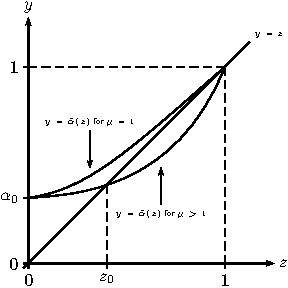
\includegraphics[width=0.5\textwidth]{figures/3.4f1.pdf}
            \end{figure}

            In other words, when $ \mu=1 $ (i.e., the so-called \emph{critical case}), there is only one root in $ [0,1] $,
            namely $ z=1 $. However, when $ \mu>1 $, there is a second root $ z=z_0\in(0,1) $ which satisfies~\ref{eq3.11}. Therefore,
            this now raises the question: \emph{Is $ \pi_0=z_0 $ or $ \pi_0=1 $ when $ \mu>1 $}?
      \item \textbf{We have}: $ z=\tilde{\alpha}(z)=\sum_{j=0}^{\infty} z^j\alpha_j\leftarrow $~\ref{eq3.11}. Let $ z=z^\star $ be any non-negative
            solution satisfying~\ref{eq3.11}. It is straightforward to show by mathematical induction that $ z^\star\ge \Prob{X_n=0} $, $ n\in\mathbb{N} $
            (left as an upcoming exercise). As a result, it follows that
            \[ \lim\limits_{{n} \to {\infty}} z^\star \ge \lim\limits_{{n} \to {\infty}} \Prob{X_n=0}\implies z^\star\ge \pi_0, \]
            which implies that $ z=\pi_0 $ is the \emph{smallest} positive number satisfying~\ref{eq3.11}. It is only when $ \mu>1 $
            (referred to as the \emph{supercritical} case) that $ \pi_0 $ is known to exist in the interval $ (0,1) $.
\end{itemize}
\begin{Example}
      \textbf{Example 3.13}. Given the following offspring probabilities, what is the probability that the
      population dies out in the long run assuming that $ X_0=1 $?
      \begin{enumerate}[(a)]
            \item $ \alpha_0=3/4 $, $ \alpha_1=1/8 $, $ \alpha_2=1/8 $.

                  \textbf{Solution}: First, we calculate
                  \[ \mu=0\biggl(\frac{3}{4}\biggr)+1\biggl(\frac{1}{8}\biggr)+2\biggl(\frac{1}{8}\biggr)=\frac{3}{8}.  \]
                  Since $ \mu<1 $, the population will die out with probability $ 1 $.
            \item $ \alpha_0=1/5 $, $ \alpha_1=1/10 $, $ \alpha_2=7/10 $.

                  \textbf{Solution}: Again, we begin by calculating
                  \[ \mu=0\biggl(\frac{1}{5}\biggr)+1\biggl(\frac{1}{10}\biggr)+2\biggl(\frac{7}{10}\biggr)=1.5. \]
                  Since $ \mu>1 $, $ \pi_0\in(0,1) $ is known to exist. To find $ \pi_0 $, we solve~\ref{eq3.11}:
                  \begin{align*}
                        z & =\tilde{\alpha}(z)                                                       \\
                        z & =\sum_{j=0}^{\infty} z^j \alpha^j                                        \\
                        z & =\frac{1}{5} +z\biggl(\frac{1}{10}\biggr)+z^2\biggl(\frac{7}{10}\biggr),
                  \end{align*}
                  giving rise to a quadratic equation
                  \[ 7z^2-9z+2=0, \]
                  or equivalently (since we know $ z=1 $ is always a solution to the above equation)
                  \[ (7z-2)(z-1)=0. \]
                  The two roots are $ z=2/7 $ and $ z=1 $. Thus, $ \pi_0=2/7 $.
      \end{enumerate}
\end{Example}
\noindent\underline{Remarks}:
\begin{enumerate}[(1)]
      \item In the case when $ X_0=n $, $ n\in\mathbb{Z}^+ $, the population will die out iff the families of each of
            the $n$ members of the initial generation die out. As a result, it immediately follows that
            the extinction probability is simply $ \pi_0^n $.
      \item For certain choices of the offspring distribution, the Galton-Watson branching process is
            not very interesting to analyse. For example, with $ X_0=1 $ and $ \alpha_r=1 $ for some $ r\in\mathbb{N} $,
            the evolution of the process is purely deterministic (i.e., $ \Prob{X_n=r^n}=1 $, $ n\in\mathbb{N} $). Another
            uninteresting case occurs when $ \alpha_0,\alpha_1>0 $ and $ \alpha_0+\alpha_1=1 $. In this situation, the
            population remains at its initial size $ X_0=1 $ for a random number of generations
            (according to a geometric distribution), before dying out completely.
\end{enumerate}
\subsection{Interesting Application \#2: The Gambler's Ruin Problem}
\begin{itemize}
      \item One of the most powerful ideas in the theory of DTMCs is that many fundamental
            probabilities and expectations can be computed as the solutions of systems of linear equations.
      \item We have already seen one such example of this through the application of the BLT\@.
      \item In what follows, we will continue to illustrate this idea by deriving appropriate linear systems
            for a number of key probabilities and expectations that arise in certain settings.
      \item To motivate this idea, let us consider a famous problem in stochastic processes known as the
            \emph{Gambler's Ruin Problem}.
\end{itemize}
\subsubsection{The Gambler's Ruin Problem}
\begin{Example}
      \textbf{Example $\bm{\pi}\approx \bm{3.14}$}. Consider a gambler who, at each play of a game, has probability $ p\in(0,1) $ of
      winning one unit and probability $ q=1-p $ of losing one unit. Assume that successive plays of
      the game are independent. If the gambler initially begins with $i$ units, what is the probability
      that the gambler's fortune will reach $N$ units ($ N<\infty $) before reaching $0$ units? This problem
      is often referred to as the \emph{Gambler's Ruin Problem}, with state $0$ representing bankruptcy and
      state $N$ representing the jackpot.
      \tcblower{}
      \textbf{Solution}: For $ n\in\mathbb{N} $, define $ X_n $ as the gambler's fortune after the $ n\textsuperscript{th} $
      play of the game, with $ X_0=i $. Clearly, $ \Set{X_n,n\in\mathbb{N}} $ is a DTMC with TPM
      \[ P=\begin{bNiceMatrix}[first-row,first-col]
                         & 0      & 1      & 2      & 3      & \cdots & N-2    & N-1    & N      \\
                  0      & 1      & 0      & 0      & 0      & \cdots & 0      & 0      & 0      \\
                  1      & q      & 0      & p      & 0      & \cdots & 0      & 0      & 0      \\
                  2      & 0      & q      & 0      & p      & \cdots & 0      & 0      & 0      \\
                  \vdots & \vdots & \vdots & \vdots & \vdots &        & \vdots & \vdots & \vdots \\
                  N-1    & 0      & 0      & 0      & 0      & \cdots & q      & 0      & p      \\
                  N      & 0      & 0      & 0      & 0      & \cdots & 0      & 0      & 1
            \end{bNiceMatrix}. \]
      Note that states $ 0 $ and $ N $ are treated as absorbing states, implying that they are both
      recurrent. States $ \Set{1,2,\ldots,N-1} $ belong to the same communication class, and it is straightforward
      to verify that it is a transient class (left as an upcoming exercise). Our goal is to determine
      $ G(i) $, $ i=0,1,\ldots,N $, which represents the probability that starting with $ i $ units, the gambler's
      fortune will eventually reach $ N $ units. As a consequence, we can deduce that
      \[ \lim\limits_{{n} \to {\infty}} P^{(n)}=\begin{bNiceMatrix}[first-row,first-col]
                         & 0        & 1      & 2      & 3      & \cdots & N-2    & N-1    & N      \\
                  0      & 1        & 0      & 0      & 0      & \cdots & 0      & 0      & 0      \\
                  1      & 1-G(1)   & 0      & 0      & 0      & \cdots & 0      & 0      & G(1)   \\
                  2      & 1-G(2)   & 0      & 0      & 0      & \cdots & 0      & 0      & G(2)   \\
                  \vdots & \vdots   & \vdots & \vdots & \vdots &        & \vdots & \vdots & \vdots \\
                  N-1    & 1-G(N-1) & 0      & 0      & 0      & \cdots & 0      & 0      & G(N-1) \\
                  N      & 0        & 0      & 0      & 0      & \cdots & 0      & 0      & 1
            \end{bNiceMatrix}. \]
      From above, note that $ G(0)=0 $ and $ G(N)=1 $ (initial conditions). Moreover, by conditioning on the outcome
      of the very first game, we readily obtain for $ i=1,2,\ldots,N-1 $:
      \begin{align*}
            G(i)                     & =p G(i+1)+q G(i-1)                    \\
            1\cdot G(i)              & =p G(i+1)+q G(i-1)                    \\
            (p+q)G(i)                & =p G(i+1)+q G(i-1)                    \\
            p G(i)+q G(i)            & =p G(i+1)+q G(i-1)                    \\
            p\bigl[G(i+1)-G(i)\bigr] & =q\bigl[G(i)-G(i-1)\bigr]             \\
            G(i+1)-G(i)              & =\frac{q}{p} \bigl[G(i)-G(i-1)\bigr].
      \end{align*}
      To determine whether an explicit solution is possible, consider several values of $ i $
      as follows:
      \begin{align*}
             & \text{Take $i=1$}\implies G(2)-G(1)=\frac{q}{p} \bigl[G(1)-G(0)\bigr]=\frac{q}{p} G(1),                    \\
             & \text{Take $i=2$}\implies G(3)-G(2)=\frac{q}{p} \bigl[G(2)-G(1)\bigr]=\biggl(\frac{q}{p}\biggr)^{\!2}G(1), \\
             & \text{Take $i=3$}\implies G(4)-G(3)=\frac{q}{p} \bigl[G(3)-G(2)\bigr]=\biggl(\frac{q}{p}\biggr)^{\!3}G(1).
      \end{align*}
      Therefore, if we take $ i=k $ we get:
      \[ G(k+1)-G(k)=\frac{q}{p} \bigl[G(k)-G(k-1)\bigr]=\biggl(\frac{q}{p}\biggr)^{\!k}G(1).\]
      Note that the above $ k $ equations are linear in terms of $ G(1),G(2),\ldots,G(k+1) $. Summing these $ k $ equations yields:
      \begin{align*}
            G(k+1)-G(1) & =\sum_{i=1}^{k} \biggl(\frac{q}{p} \biggr)^{\! i}G(1)                                   \\
            G(k+1)      & =\sum_{i=0}^{k} \biggl(\frac{q}{p} \biggr)^{\! i}G(1),\text{ for $ k=0,1,\ldots,N-1 $},
      \end{align*}
      or equivalently,
      \[ G(k)=\sum_{i=0}^{k-1}\biggl(\frac{q}{p} \biggr)^{\! i}G(1),\text{ for $ k=1,2,\ldots,N $}. \]
      Applying the formula for a finite geometric series, we end up with
      \[ G(k)=\begin{dcases}
                  \frac{1-(q/p)^k}{1-(q/p)}G(1), & \text{if $p\ne 1/2$}, \\
                  k G(1),                        & \text{if $p=1/2$}.    \\
            \end{dcases} \]
      Plugging in $ k=N $, we obtain for $ p\ne 1/2 $:
      \[ 1=G(N)=\frac{1-(q/p)^N}{1-(q/p)}G(1)\implies G(1)=\frac{1-(q/p)}{1-(q/p)^N}.  \]
      Similarly, for $ p=1/2 $, we obtain:
      \[ G(1)=\frac{1}{N}. \]
      Combining both cases, we ultimately get for $ k=1,2,\ldots,N $.
      \[ G(k)=\begin{dcases}
                  \frac{1-(q/p)^k}{1-(q/p)^N}, & \text{if $ p\ne 1/2 $}, \\
                  \frac{k}{N},                 & \text{if $p=1/2$}.
            \end{dcases} \]
      In fact, this holds for $ k=0,1,2,\ldots,N $.
\end{Example}
\noindent\underline{Remarks}:
\begin{enumerate}[(1)]
      \item An interesting question to ask is what happens to the gambler's probability of winning the
            jackpot, given an initial fortune of $i$ units, as $N$ grows ``larger'' (i.e., $ N\to\infty $)? In other
            words, what happens to the limit of $G(i)$ as $ N\to\infty $. Looking at three cases based on
            the value of $p$, we see:
            \begin{enumerate}[(i)]
                  \item When $ p=1/2 $, $ G(i)=\dfrac{i}{N} \to 0 $ as $ N\to\infty $,
                  \item When $ p<1/2 $, $ G(i)=\dfrac{1-(q/p)^i}{1-(q/p)^N}\to 0 $ as $ N\to\infty $,
                  \item When $ p>1/2 $, $ G(i)=\dfrac{1-(q/p)^i}{1-(q/p)^N}\to 1-\biggl(\dfrac{q}{p}\biggr)^{\! i} $ as $ N\to\infty $,
            \end{enumerate}
            since $ q/p>\text{($<$)}1 $ when $ p<\text{($>$)}1/2 $. Simply put, only when $ p>1/2 $ does a positive
            probability exist that the gambler's fortune will increase indefinitely. Otherwise, the
            gambler is sure to go broke.
      \item In our study of the \emph{Random Walk} in Example 3.9 featuring a DTMC on the state space $ \mathbb{Z} $
            with transition probabilities analogous to those in the \emph{Gambler's Ruin Problem}, we
            previously showed that
            \[ f_{0,0}=(1-p)f_{-1,0}+pf_{1,0}. \]
            Suppose that $ p>1/2 $. First, note that
            \begin{align*}
                  f_{1,0}
                   & =\Prob{\text{Random Walk DTMC ever makes a future visit to state $0$ starting from state $1$}}     \\
                   & =\lim\limits_{{N} \to {\infty}}\Prob{\text{Gambler's Ruin DTMC ends up in bankruptcy}\given X_0=1} \\
                   & =1-\Biggl(1-\biggl(\frac{1-p}{p} \biggr)^{\!1}\Biggr)\text{ from case (iii) of Remark (1)}         \\
                   & =\frac{1-p}{p}.
            \end{align*}
            Similarly, we also have that
            \begin{align*}
                  f_{-1,0}
                   & =\Prob{\text{Random Walk DTMC ever makes a future visit to state $0$ starting from state $-1$}}                                  \\
                   & =\lim\limits_{{N} \to {\infty}}\Prob{\text{Gambler's Ruin DTMC with ``up'' probability $1-p$ ends up in bankruptcy}\given X_0=1} \\
                   & =1-0\text{ from case (ii) of Remark (1) since $1-p<1/2$}                                                                         \\
                   & =1.
            \end{align*}
            Therefore, we end up ultimately obtaining
            \[ f_{0,0}=(1-p)\cdot 1+p\biggl(\frac{1-p}{p}\biggr)=2(1-p), \]
            which agrees with our earlier result. The same essential procedure can be adapted to verify
            that $ f_{0,0}=2p $ if $ p<1/2 $.
\end{enumerate}